% Vertical Line Title Page
% LaTeX Template
% Version 2.0 (22/7/17)
%
% This template was downloaded from:
% http://www.LaTeXTemplates.com
%
% Original author:
% Peter Wilson (herries.press@earthlink.net) with modifications by:
% Vel (vel@latextemplates.com)
%
% License:
% CC BY-NC-SA 3.0 (http://creativecommons.org/licenses/by-nc-sa/3.0/)

\documentclass{article}
\usepackage[utf8]{inputenc}
\usepackage{hyperref}
\usepackage{graphicx}

\begin{document}
%---------------------------------------------------------------------------------
%	TITLE PAGE
%--------------------------------------------------------------------------------

\begin{titlepage} % Suppresses displaying the page number on the title page and the subsequent page counts as page 1
	
	\raggedleft % Right align the title page
	
	\rule{1pt}{\textheight} % Vertical line
	\hspace{0.05\textwidth} % Whitespace between the vertical line and title page text
	\parbox[b]{0.75\textwidth}{ % Paragraph box for holding the title page text, adjust the width to move the title page left or right on the page
		
		{\Huge\bfseries Elaboration \\[0.5\baselineskip] Assignment}\\[2\baselineskip] % Title
		{\large\textit{Planning and Testing}}\\[4\baselineskip] % Subtitle or further description
		{\Large\textsc{Emily Hunt 44888619}} % Author name, lower case for consistent small caps
		
		\vspace{0.5\textheight} % Whitespace between the title block and the publisher
		}

\end{titlepage}


View in Overleaf: \url{https://www.overleaf.com/read/bkhpthjqbtdr}

\tableofcontents

\pagebreak

\section{Scoping II Decomposition}
I realised I partially misunderstood the expectation for decomposition last week (my response for this section was more appropriate for the algorithm section). So I will first re-attempt decomposition, by breaking down my usual process for analysing the colour of films.

\begin{enumerate}
    \item I watch a film in its entirety taking notes on the colour palette used and how various colours are used thematically. These will most likely \textbf{not} be labelled very clearly (e.g. with time stamps) but just be general notes.
    \item When reviewing these notes to write an essay etc., I will have to go back through the film and try and work out which part of it the notes are referencing, which can be a very time consuming and fiddly process.
\end{enumerate} 

Using the XY Problem resource (\url{http://xyproblem.info/}), I also realised that my issue was not solely analysing the colour of films, but organising my notes concerning these. Therefore, the technologies listed below to accomplish each step in the decomposition will be divided into those that assist with colour analysis, and note taking. These will be evaluated in terms of what Brian noted on Slack to be signs of a good tool (well written and easily understandable documentation, as well as recent maintenance (indicating wide use)).

\section{PLANNING}

\subsection{Solutions for Colour Analysis}
I couldn't really find a tool that did specifically what I identified in scoping (measures the number of times a colour appears throughout a film), so I switched my focus to tools that would create a colour map of a film.

\subsubsection{GitHub: Cinemetrics (Original)}
URL: \url{https://github.com/freder/cinemetrics}\\
This tool would be ideal, as in addition to producing a map of the colours present in a film, it provides a representation of a number of the film's other features, such as shot duration and motion, which are things I hadn't really considered before. However, this tool will probably not be viable to use, as it fails to meed a number of the criteria identified on Slack: 
\begin{itemize}
    \item Documentation: There is no documentation provided with this tool, as explicitly noted on its GitHub repository.
    \item Maintenance: The last commits for this project were 8/9 years ago.
\end{itemize}

\subsubsection{GitHub: Cinemetrics}
URL: \url{https://github.com/suite22/cinemetrics}\\
This tool is a different version of the previously identified one. It seems more feasible than the other option in one respect:

\begin{itemize}
    \item Documentation: Detailed documentation is provided with this tool. From a preliminary reading, it seems to be understandable.
    \item Maintenance: However, similarly to the aforementioned tool, a number of the latest commits for a number of the files were 8 years ago, though a few were as recent as 3/4 years ago.
\end{itemize}
I did an initial test of this software. I installed vagrant as instructed, downloaded a zip of the repository and then in Terminal, made the copy of the repository the working directory and entered 'vagrant up'. This produced a message informing me I needed to install a 'provider', with VirtualBox recommended. However, I had some issues with security and privacy settings when trying to install VirtualBox, so stopped the test here.

\subsubsection{GitHub: Colors-of-Film}
URL: \url{https://github.com/sacert/Colors-of-Film}\\
This tool may also prove to be a viable option. It allows customisation of the size (length/width) of the output colour map image.
\begin{itemize}
    \item Documentation: The documentation is very straightforward and clear, and it seems the software is simple to use.
    \item Maintenance: The last commits were 2/3 years ago, and the repository has 16 stars.
\end{itemize}

\subsubsection{GitHub: FilmStrip}
URL: \url{https://github.com/ArkadiusBear/FilmStrip}\\
The tool may also be viable for producing a colour map of a film. At allows the customisation of a number of aspects of the output image, including size, ratio and density.

\begin{itemize}
    \item Documentation: Really clear documentation is provided regarding what the tool does and how it works, though there doesn't appear to be much documentation in relation to how to use the tool.
    \item Maintenance: The last commits were 8 months ago, making this the most recently updated repository of all the tools listed. However, these commits were only over two days, indicating there has not been a long process of testing and updating.
\end{itemize}
 
\subsection{Solutions for Note Taking}
URL: \url{http://www.clipnotes.org/}\\
Though I can't locate the code for this tool, it seems like it could be a really valuable tool. It appears that for it to work, you download the app, have a film file and your notes (with a time stamp) in an XML file. You can then open the film file and notes in the app, and it will display the notes at the appropriate time in the film.
\begin{itemize}
    \item Documentation: There is really detailed documentation on how to use the software on the website, as well as a trouble shooting section.
    \item Maintenance: From what I can see, the last update of the software was 2015.
\end{itemize}

This solution could be potentially combined with one of the colour analysis solutions, so that a specific portion of the colour map could be linked (through the XML file?) to that specific section of the film if I want to view it in more detail.

\subsection{Inspiration}

The inspiration for the potential combination for these two tools came from an app called 'Animated' by Walt Disney Animation Studios. It includes a colour map of each of the studio's films which you can select and scrub through to see certain stills (\autoref{fig:colourmaps}). While this is useful to me in its current form (as I plan to analyse Disney films in my thesis) the production of colour maps is something I would like to learn how to do for potential future studies. Furthermore, in their current form the colour maps in this app are difficult to navigate as it is really fiddly to select and scrub through a specific film. I would like to be able to have a colour map and go that section of the film to look at in more detail, while also being able to see the notes I have written, which is what I am proposing in this elaboration.

\begin{figure}[htp]
    \centering
    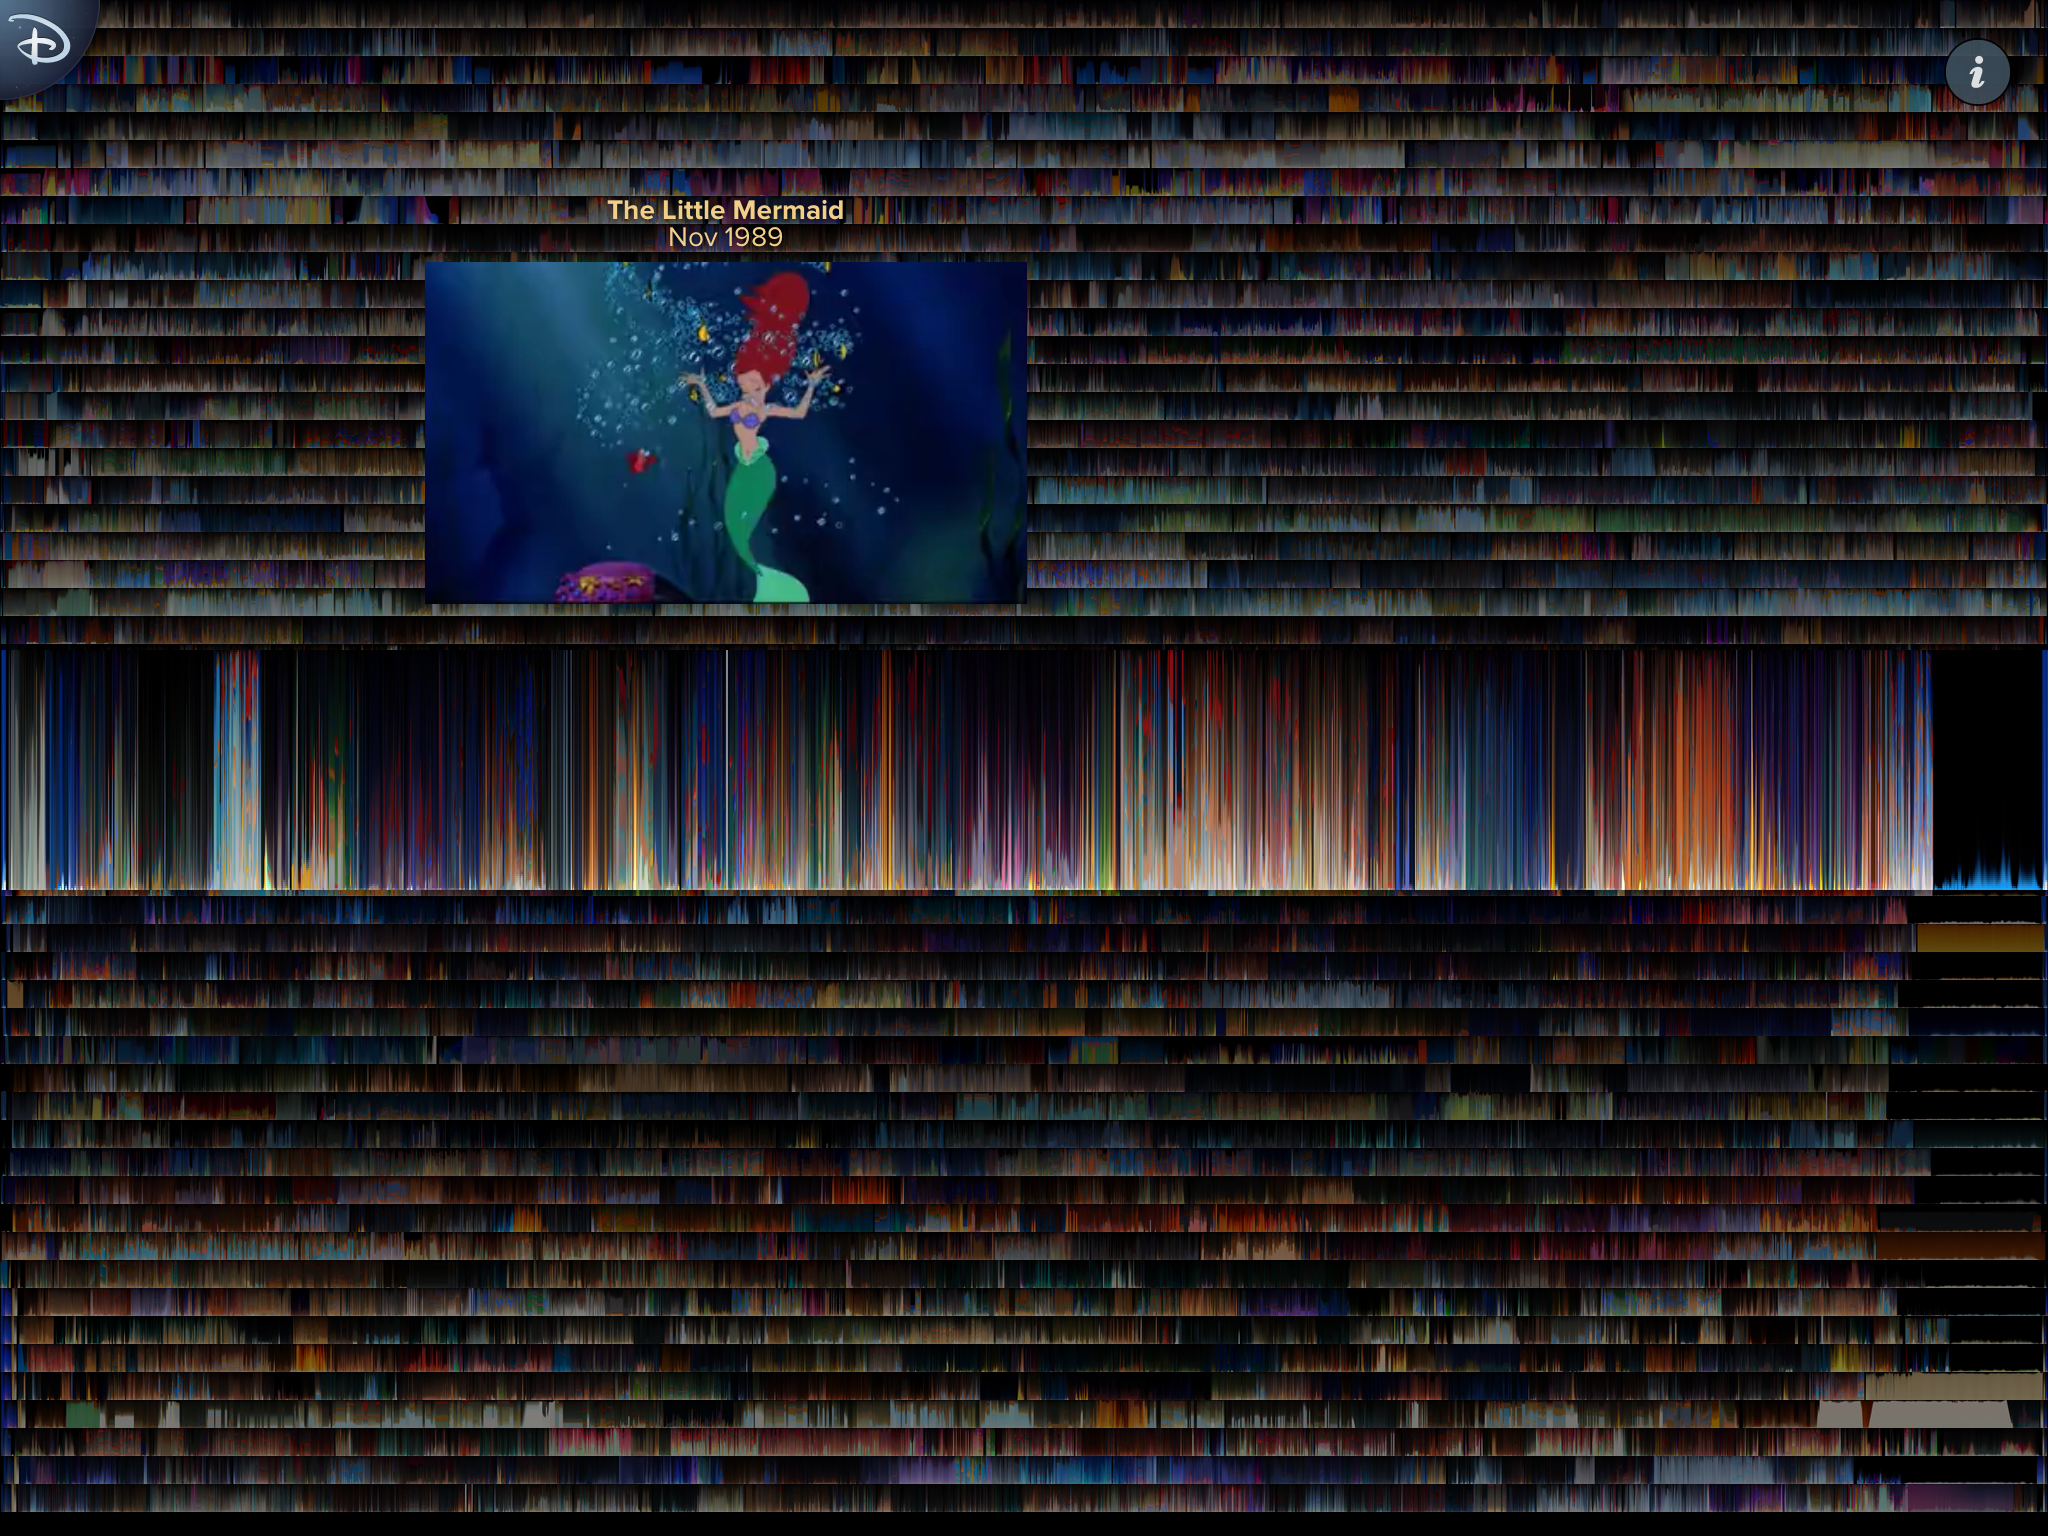
\includegraphics[width=6cm]{IMG_9495.PNG}
    \caption{Colour Maps of Disney Films in the 'Animated' App}
    \label{fig:colourmaps}
\end{figure}

\pagebreak

\section{TESTING}

To test each of these solutions, I used a 3 minute video I had taken on my iPhone of a parade. This was chosen because I thought using a smaller video file (rather than a full length film) would allow me to test the solutions more quickly, and I still have to think about sourcing the full length films and potential copyright considerations. I also placed a one hour limit on the tests for each of the different tools.

\subsection{Solutions for Colour Analysis}

\subsubsection{GitHub: ACTION-Video-Toolkit}
URL: \url{https://github.com/bregmanstudio/ACTION-Video-Toolki}\\
Since completing the planning stage of elaboration, I found this additional tool. If successful, it would be absolutely ideal for my completing my thesis, as it supposedly provides a toolkit to analyse similarities across films. I consulted Brian on Slack for how to begin the testing for this tool.\\

\textbf{Objective:}\\
\textbf{Time Stamp:} text\\
\textbf{Actions:} text\\
\textbf{Results:} text\\
\textbf{Errors} text\\
\textbf{Solutions/Notes} text\\

\subsubsection{GitHub: Cinemetrics}
URL: \url{https://github.com/suite22/cinemetrics}\\
text

\subsubsection{GitHub: Cinemetrics}
URL: \url{https://github.com/suite22/cinemetrics}\\
text

\subsubsection{GitHub: Colors-of-Film}
URL: \url{https://github.com/sacert/Colors-of-Film}\\

\textbf{Objective: Try Running the Python Script}\\
\textbf{Time Stamp:} 11:45am 3 September\\
\textbf{Actions:} The information on the GitHub page said I needed Numpy and OpenCV, but I wanted to just see what happened if I tried to run it. I downloaded the GitHub Repository as a zip, unzipped the folder and moved it to my desktop. I then moved the file I wanted to trial the python script on into the folder using GUI, and then made this the working directory in the Unix Shell. As instructed, I entered, 'python colorsOfFilm.py Test.mov 50 30'.\\
\textbf{Errors} This produced the message File "colorsOfFilm.py", line 2, in <module>; import cv2;ImportError: No module named cv2\\
\textbf{Solutions/Notes:} I then tried to install OpenCV.\\

\textbf{Objective: Install OpenCV}\\
\textbf{Time Stamp:} 12:06pm 3 September\\
\textbf{Actions:} I went to \url{https://opencv.org/} and clicked learn more under 'OpenCV 4.1.1 The latest release is now available'. Under OpenCV – 4.1.1, I clicked iOS pack, which took me to SourceForge where a zip file started automatically downloading. I unzipped the file\\
\textbf{Results:} text\\
\textbf{Errors} text\\
\textbf{Solutions/Notes} text\\

\textbf{Objective: Install Numpy}\\
\textbf{Time Stamp:} text\\
\textbf{Actions:} text\\
\textbf{Results:} text\\
\textbf{Errors} text\\
\textbf{Solutions/Notes} text\\

\subsubsection{GitHub: FilmStrip}
URL: \url{https://github.com/ArkadiusBear/FilmStrip}\\
text

\subsection{Solutions for Note Taking}
URL: \url{http://www.clipnotes.org/}\\

\textbf{Objective: Download ClipNotes App to My iPad}\\
\textbf{Time Stamp:} 1:35pm 3 September\\
\textbf{Actions:} On my iPad, I went into the App Store and searched Clip Notes. I clicked GET and then INSTALL on the appropriate app (the icon with the film strip down the middle and a paper clip).\\
\textbf{Results:} The app was installed successfully. I opened the app and viewed the example film and notes. If you clicked on a specific note, it was expanded under the viewing window and it played the specific part of the film the note referred to, stopping at the end timestamp. You select Change Film to switch to a different film you have saved to the app or Cahnge Notes to different notes you have saved. As I didn't have another film or notes I couldn't change these.\\
\textbf{Errors:} None.\\
\textbf{Solutions/Notes:} You cannot use films saved to your iPad in iTunes, you have to save them to the app from iTunes on your computer (as it says on the site).\\

\textbf{Objective: Create a XML File with My Notes}\\
\textbf{Time Stamp:} 1:45pm 3 September\\
\textbf{Actions:} I checked the ClipNotes website and TextWrangler which I already had installed on my computer was listed as an XML editor to use. So I created a file with notes for two sections of the film (with a caption and description) using the template from the ClipNotes site, and saved the file on my desktop.\\
\textbf{Results:} The file was successfully saved, but as a .txt file, which caused me issues later. \\
\textbf{Errors:} I encountered an error when trying to open this file in the app. \\
\textbf{Solutions/Notes:} Please see Error: Notes File Causing the App to Crash for solutions to this error.\\

\textbf{Objective: Transfer Video and Notes Files to iPad from Computer}\\
\textbf{Time Stamp:} 1:52pm 3 September\\
\textbf{Actions:} I connected my iPad to my computer using a lightning to USB cable. iTunes opened automatically, and I selected the iPad symbol near the top menu bar. In the page this opened, in the left menu bar I selected 'File Sharing' (it has the little 'A' symbol next to it like the App Store logo). Under Apps, I selected ClipNotes, and dragged and dropped the appropriate files into the space for files (I could have also clicked the Add button).\\
\textbf{Results:} These were successfully transferred onto my iPad after a short period.\\
\textbf{Errors:} None. \\
\textbf{Solutions/Notes:}\\

\textbf{Objective: Open Video and Notes in App}\\
\textbf{Time Stamp:} 2:00pm 3 September\\
\textbf{Actions/Results:} Within the app, I selected Change Film. The one I had transferred to my iPad appearred, I selected it and it was successfully loaded in the viewing window.\\
\textbf{Errors:} However, when I selected Change Notes, the app crashed. When I quit the app and then tried to reopen it the app would not open at all.\\
\textbf{Solutions/Notes:} Please see the next Error.\\

\textbf{Error: Notes File Causing the App to Crash}\\
\textbf{Actions:} I realised my issue was a result of the file not being in an XML format. After some searching online, the most frequently suggested solution to my problem was, within TextWrangler, selecting Text in the menu bar, and then Apply Text Filter. However, TextWrangler would not allow me to select this option. I then tried creating an XML file from the Unix Shell, by entering 'nano test.xml' with the Desktop as my working directory. When transfered to my iPad, this still caused the app to crash. I also tried just changing the extension of the file from .txt to .xml which didn't work either (I know we were told not to do this in class but I wanted to exhaust all options). I then looked at the Troubleshooting section of the ClipNotes website which informed me a common problem was problems in the XML files (such as not correctly closing a tag). From this, I realised I had not correctly closed my main \verb|<\Clips>| tag. I then addressed this issue in the file I had created in the Unix Shell but this still caused the app to crash. I then went to the XML Database of film notes on the ClipNotes website. I selected the notes for the film \textit{Contempt} (A random choice) which opened in a new tab. I then selected File in the menu tab and selected Save. In the window that opened, the format of the file was 'XML text'. I saved the file to my desktop and transferred it to my iPad. The app opened and the notes for the film opened successfully with the video I had transferred. On my computer, I then edited the \textit{Contempt} notes files to be notes for my own video, and then transferred this to my iPad, and these opened successfully with the video on the app, playing the correct portions of the video with the corresponding notes.

\subsection{Solutions for Script Analysis}

Agile - response

Explanation

URL: \url{http://www.scripthreads.org/}\\

\textbf{Objective: Install and Open the Script Threads Application on My Computer}\\
\textbf{Time Stamp:} 9:30pm 3 September\\
\textbf{Actions:} text\\
\textbf{Results:} text\\
\textbf{Errors:} text\\
\textbf{Solutions/Notes:} text\\

find script - html format 
\url{https://www.dailyscript.com/}
I just downloaded the first one under movies - 10 things I hate about you
check file download time

open in app - automatically did it

characters - made my own - check creation of file
go through how I did it


\end{document}